\chapter{Optimal Block Production Problem}
\label{chp:mining}
This chapter originally appeard in the following publications:

\begin{itemize}

    \item T. Barakbayeva, S. Farokhnia, A.K. Goharshady, S. Novozhilov, Boosting Gas Revenues of Ethereum Miners, IEEE/ACM International Conference on Software Engineering, ICSE 2026
    \item T. Barakbayeva, S. Farokhnia, A.K. Goharshady, M. Gufler, S. Novozhilov, Pixiu: Optimal Block Production Revenues on Cardano, IEEE International Conference on Blockchain, Blockchain 2024
\end{itemize}


\newpage

\section{Introduction}

\para{Background} In modern cryptocurrencies, a blockchain is a linked-list of blocks, which in turn contain a sequence of transactions. Anyone on the network can create and broadcast a transaction, but the transaction is only considered finalized when it is added to the blockchain. The blockchain is subject to consensus, i.e.~all nodes on the network will eventually agree on its contents. The consensus mechanism varies by cryptocurrency. For example, Bitcoin uses proof of work, whereas Ethereum runs on proof of stake. Irrespective of this, all modern cryptocurrencies heavily rely on miners. These are nodes who actively partake in running the consensus mechanism and extending the blockchain by adding new blocks. To incentivize the miners to add new transactions to the blockchain, each transaction includes a fee, which is paid to the miner who includes it in her block. This setting creates a natural optimization problem from the point-of-view of miners: Given a set of new transactions which are not yet added to the blockchain, how can we form an optimal block that maximizes the fees and thus the miner's revenue?


In this chapter, we address this optimization problem for two mainstream cryptocurrencies:
\begin{enumerate}
    \item \textbf{Cardano:} A blockchain protocol based on proof-of-stake and an extended UTXO model which also supports arbitrary smart contracts. Its primary currency, Ada, is currently one of the global top ten cryptocurrencies with a market cap of more than 16 billion USD. In Cardano, new blocks are produced by stake pools. Any holder of Ada can delegate their stake to a pool. The underlying proof-of-stake consensus protocol is Ouroboros Praos, which divides time into a number of epochs and each epoch into a number of slots, each corresponding to one second. In each slot, leaders are randomly selected to produce and add new blocks to the blockchain, with their selection probability being proportional to their stake. Each block can contain a sequence of transactions and block production is rewarded in two ways: (i)~transaction fees and (ii)~monetary expansion. The producers have no control over (ii), but can optimize (i) by choosing which transactions to include in their blocks. Thus, they are incentivized to maximize the total transaction fees.

    \item \textbf{Ethereum:} Currently world's largest programmable blockchain by market cap. On Ethereum, the fees depend on the execution costs of the transaction. Given that Ethereum supports arbitrary smart contracts in a Turing-complete language, the fee paid by a transaction can depend on the context in which it is executed, which is determined by the set of transactions that precede it on the blockchain. Thus, the problem becomes considerably more challenging. An Ethereum miner who wishes to maximize her revenue has to choose not only a subset of transactions to include in her block, but also their exact order. Moreover, each permutation of the same transactions might change the amount of fee paid by each transaction. This causes a combinatorial explosion.

\end{enumerate}
  		
	

\para{Our Contributions} This chapter provides algorithms and empirical results for optimal block production on Cardano and Ethereum:

\begin{enumerate}
    \item \textbf{Cardano.} In Section~\ref{sec:mining-cardano-problem}, we formalized the block production problem on Cardano. Then, in Section~\ref{sec:mining-cardano-algorithm}, we show that by exploiting the sparsity of interrelations between transactions, i.e.~the small treedepth of dependency-conflict graphs, it is possible to obtain a polynomial-time algorithm that outputs optimal blocks. In Section~\ref{sec:mining-cardano-experiments}, we implemented our algorithm in a free and open-source tool called Pixiu. Using Pixiu, we provide extensive experimental results over real-world transaction data on the Cardano blockchain, demonstrating that our approach increases the block producers' revenue by almost 1,357.82 USD/day (= 495,604.3 USD/year).

    \item \textbf{Ethereum.} Sections~\ref{sec:mining-ethereum-problem} and~\ref{sec:mining-ethereum-algorithm} study the block production problem for Ethereum and introduce a randomized framework for increasing miners' transaction-fee revenues. The framework combines testing, decision trees, integer linear programming, and localization techniques to ameliorate the combinatorial explosion. Finally, Section~\ref{sec:mining-ethereum-experiments} reports significant empirical gains: our method outperforms real-world Ethereum miners by an average of 73.45\% per block, corresponding to roughly 63 million USD per annum.
\end{enumerate}




% Cardano Mining Paper
\section{Cardano eUTXO Model}\label{sec:mining-cardano-problem} 


In general, block producers in Cardano have no control over the monetary expansion component of the protocol rewards. However, they can choose which transactions to include in their blocks, thereby exercising some control over transaction fees. Block producers are collectively incentivized to maximize the total amount of transaction fees in their epoch and thus in their block. See Section~\ref{sec:prelim-cardano} for a comprehensive overview of Cardano's architecture.
In this section, we focus on solving the problem of forming an optimal block on the Cardano blockchain. Specifically, given a set of unmined transactions, i.e.~transactions that are not yet added to the blockchain, our goal is to create a valid Cardano block with the maximum possible amount of transaction fees, thus maximizing the total revenue of block producers.



\para{Optimal Block Production} Given a block size limit $k \in \mathbb N,$ a finite set $\txs$ of $n$ unmined Cardano transactions in which every transaction $t \in \txs$ has a set of inputs, a set of outputs, a fee $\cfee(t) \in [0, \infty)$ and a size $\sz(t) \in \mathbb{N},$ find a subset $\txs^\ast \subseteq \txs$ of transactions such that:
\begin{itemize}
	\item $\txs^\ast$ satisfies all the dependency and conflict requirements as above;
	\item $\sum_{t \in \txs^\ast} \sz(t) \leq k,$ i.e.~all the chosen transactions fit into the block size limit; and
	\item $\sum_{t \in \txs^\ast} \cfee(t)$ is maximized, i.e.~the block consisting of the transactions in $\txs^\ast$ yields the maximum possible total transaction fee.
\end{itemize}
In practice, we always have $k=90112.$

\para{Dependency-Conflict Graphs (DCGs)~\cite{meybodi2022optimal}} Given an instance of the optimal block production problem above, we create a graph $G = (\txs, E_C \cup E_D)$ in which there is a vertex corresponding to every transaction in $\txs$ and an undirected edge $\{t_1, t_2\} \in E_C$ whenever the transactions $t_1$ and $t_2$ are in conflict, as well as a directed edge $(t_1, t_2) \in E_D$ when transaction $t_2$ depends on transaction $t_1.$ See Figure~\ref{fig:mining-cardano-dcg}.

\begin{figure}[H]
	\centering
	\includegraphics[scale=0.65]{chapters/mining/mining-cardano-figures/tdpGraph.pdf}
	\caption{An example dependency-conflict graph. Dependency edges are shown in blue and conflict edges in red.}
	\label{fig:mining-cardano-dcg}
\end{figure}

The work~\cite{meybodi2022optimal} (IEEE Blockchain 2022) considered DCGs in the context of Bitcoin mining. It showed that if the DCGs are sparse and path-like, then the optimal block production problem for Bitcoin is efficiently solvable. The approach in~\cite{meybodi2022optimal} depends on the concepts of pathwidth and path decompositions. Intuitively, it first computes a decomposition of the DCG into a path and then uses a dynamic programming algorithm to obtain the optimal block. Unfortunately, such an approach is too slow and not applicable to our use-case in Cardano. This is because in Cardano, a new block has to be produced every second,  whereas computing the decomposition notion used in~\cite{meybodi2022optimal} takes minutes. This was not a problem in Bitcoin, where a new block is added every 10 minutes, but is not scalable enough for Cardano. Therefore, in this problem, we consider a stronger notion of decomposition, namely the treedepth decomposition, and provide an algorithm based on treedepth to solve the optimal block production problem in Cardano. As we will see in Section~\ref{sec:mining-cardano-experiments}, our algorithm is highly scalable in practice and produces optimal blocks in less than a second, hence enabling its application in Cardano.



\subsection{Treedepth}

\para{Treedepth Decompositions~\cite{nevs2012bounded, iwata2017power, nevs2015low}} For a graph $G= (V, E),$ a \emph{treedepth decomposition} is a rooted tree $T = (V, E_T)$ on the same set of vertices as $G$ that satisfies the following requirement:
\begin{itemize}
	\item For every undirected edge $\{u, v\} \in E$ or directed edge $(u, v) \in E$ of the original graph, either $u$ is an ancestor of $v$ in $T$ or $v$ is an ancestor of $u$ in $T.$
\end{itemize}
We say that a treedepth decomposition $T$ is optimal if it has the smallest possible depth among all decompositions of $G.$ This smallest depth is called the \emph{treedepth} of $G.$ Intuitively, treedepth is a measure of graph sparsity that captures how much a graph resembles a shallow tree. Throughout this problem, we always consider the treedepth $d$ of a dependency-conflict graph $G.$ See Figure~\ref{fig:mining-cardano-deco}.

\para{Computing Treedepth} For any small fixed $d,$ there is an algorithm that decides whether an input graph has treedepth $d$ in linear time and if so, outputs an optimal treedepth decomposition~\cite{reidl2014faster}. There are also well-optimized tools and libraries for computing treedepth decompositions~\cite{strasser2020pace}. As we will see in Section~\ref{sec:mining-cardano-experiments}, DCGs in Cardano have small treedepth. Thus, in the remainder of this chapter we assume, without loss of generality, that we have access to an optimal treedepth decomposition of every DCG. In practice, we use~\cite{strasser2020pace} to find such decompositions.

\para{Vertex Numbering} Recall that the vertices in our DCGs are unmined Cardano transactions. We number the vertices by a pre-order (left-to-right) traversal of our treedepth decomposition. See Figure~\ref{fig:mining-cardano-deco} as an example. This is also without loss of generality, but allows us to present our algorithm more concisely. 

\begin{figure}
	\begin{center}
		\includegraphics[scale=0.65]{chapters/mining/mining-cardano-figures/tdpDec.pdf}
	\end{center}
\caption{A treedepth decomposition of the DCG graph of Figure~\ref{fig:mining-cardano-dcg}. The edges of the decomposition are dashed. Every edge of the original graph (shown in red and blue) goes between a vertex and one of its ancestors. The vertices are numbered in pre-order. This decomposition has a depth of $3,$ since the path from the root $1$ to the farthest leaf $5$ has three edges.}
\label{fig:mining-cardano-deco}
\end{figure}

\para{Ancestor Sets} Suppose that our treedepth decomposition $T$ is rooted at vertex $1$. For every vertex $v \in V,$ we denote by $A_v$ the set of ancestors of $v,$ i.e.~the set of vertices that are on the path from the root $1$ to $v$ in $T.$ For two vertices $u, v \in V,$ we define $A_{u, v} := A_u \cap A_v$ as the set of their common ancestors, i.e.~vertices that are ancestors of both $u$ and $v.$ Since we numbered the vertices in pre-order, we have $A_{i, i-1} = A_i \setminus \{i\}$ for every vertex $i.$
\section{Treedepth-Based Optimal Block Construction for Cardano}\label{sec:mining-cardano-algorithm} 

In this section, we present our algorithm for finding an optimal Cardano block that maximizes the total transaction fee revenue of the block producers. Our algorithm is a dynamic programming approach based on the treedepth decomposition of the conflict-dependency graph of our unmined transactions.

\para{Input} Suppose that we are given an optimal block production instance, consisting of the block size limit $k \in \mathbb N$ and a set $\txs$ of $n$ unmined Cardano transactions as input. Each transaction $t \in \txs$ has a fee of $\cfee(t)$ and a size of $\sz(t).$ Additionally, we have the dependency-conflict graph $G = (\txs, E_C \cup E_D)$ and a treedepth decomposition $T = (\txs, E_T)$ of $G$ with depth $d.$ Our goal is to solve the optimal block production problem.

\para{Canonical Subgraphs} We define $n$ canonical subgraphs of our DCG $G.$ The $i$-th canonical subgraph $G_i$ consists of the first $i$ transactions, as well as any conflicts and dependencies between them. Formally, we let
$$
V_i = \{1, 2, \dots, i\}
$$
and
$$
G_i = G[V_i].
$$
Recall that the transactions are numbered by a pre-order traversal of $T.$ We consider subproblems on each $G_i = (V_i, E_i)$ and show how to combine the results on these subproblems to find an optimal block for the entire DCG $G.$ See Figure~\ref{fig:mining-cardano-cano}.

\begin{figure*}
	\centering
	\includegraphics[width=\linewidth]{chapters/mining/mining-cardano-figures/canon.pdf}
	\medskip
	\caption{Canonical subgraphs of the graph $G$ of Figure~\ref{fig:mining-cardano-dcg} based on the treedepth decomposition of Figure~\ref{fig:mining-cardano-deco}. In each $G_i,$ the set $A_i$ of ancestors of vertex $i$ is shown in blue.}
	\label{fig:mining-cardano-cano}
\end{figure*}

\para{Dynamic Programming Table} For every $1 \leq i \leq n,$ every partial capacity $0 \leq c \leq k$ and every subset $S \subseteq A_i,$ we define a subproblem and a dynamic programming variable as follows:
$$
\hspace{-1em}\begin{array}{rl}
\dpt[i, S, c] := & \text{The maximum total fees } \Sigma_{t \in \txs^\ast} \cfee(t)\\
& \text{ of a set } \txs^\ast \subseteq V_i \text{ of transactions in } G_i\\
& \text{ such that } \txs^\ast \cap A_i = S\\
& \text{ and } \Sigma_{t \in \txs^\ast} \sz(t) \leq c\\
& \text{ and } \txs^\ast \text{ satisfies dependencies/conflicts in } E_i.
\end{array}
$$
Intuitively, we are considering subproblems in which we have only the first $i$ vertices/transactions and their dependencies/conflicts, but we also consider the case where our capacity is $c \leq k,$ i.e.~part of the block is already filled and we only have $c$ bytes of free space remaining. Finally, the set $S$ tells us exactly which ancestors of transaction $i$ should be taken into the solution.

\para{Computing Values for $G_1$} The subgraph $G_1$ consists only of the root vertex $1$ and has no edges. Thus, we have 
$$
\dpt[1, \emptyset, c] = 0,
$$
and
$$
\dpt[1, \{1\}, c] = \left\{\begin{matrix}
	\cfee(1) & \sz(1) \leq c \\
	-\infty & \sz(1) > c \\
\end{matrix}\right. .
$$
We use $-\infty$ to show an impossible situation, i.e.~when no possible set $\txs^\ast$ satisfying the requirements can be found.

\para{Computing Values for Other $G_i$'s} Suppose $i > 1$ and we intend to compute $\dpt[i, S, c].$ Moreover, assume that the $\dpt[j, \cdot, \cdot]$ values are already computed for all $j < i.$
\begin{itemize}
	\item We first check if $S$ violates any of the dependency and conflict requirements in the set $A_i,$ i.e.~between the ancestors of vertex $i.$ Specifically, for any two vertices $u, v \in A_i,$ if $\{u, v\} \in E_C$ and also $u, v \in S,$ then they are in conflict but both taken in $S$ and so we have to set $\dpt[i, S, c] = -\infty$ since the requirements are impossible to satisfy. Similarly, if $(u, v) \in E_D$ and $v \in S$ but $u \not\in S,$ then the dependency requirement is violated and we set $\dpt[i, S, c] = -\infty.$ For example, in Figure~\ref{fig:mining-cardano-cano} we set $\dpt[4, \{4\}, 10]$ to $-\infty$ since $4$ is included and depends on $2,$ which is not included. Similarly, $\dpt[3, \{1, 2, 3\}, 10] = -\infty$ since $1$ and $3$ are in conflict.
	\item We then check if all the transactions in $S$ can fit into $c$ bytes, i.e.~whether $\sum_{t \in S} \sz(t) \leq c.$ If not, we set  $\dpt[i, S, c] = -\infty.$
	\item Let $S' \subseteq A_{i-1}$ be a subset of ancestors of vertex $i-1.$ We say that $S'$ is \emph{compatible} with $S$ and write $S' \leftrightarrows S$ if $\forall u \in A_{i-1, i}$ we have $u \in S \Leftrightarrow u \in S'.$ In other words, compatible subsets make the same decisions about the common ancestors of $i$ and $i-1.$ If all the checks above pass, then we consider two cases:
	\begin{enumerate}[label=(1)]
		\item If $i \not\in S,$ then we know that our solution $\txs^\ast$ cannot contain the transaction $i.$ Thus, all transactions in the solution are already present in $G_{i-1}$.
		
		 Therefore, we set $$\dpt[i, S, c] = \max_{S' \leftrightarrows S} \dpt[i-1, S', c].$$
		\item If $i \in S,$ then we must put the transaction $i$ into our solution $\txs^\ast.$ This reduces the available space to $c - \sz(i)$ but also gives us a fee of $\cfee(i).$ We should then fill out our block using the previous $i-1$ transactions. Thus, we have
		$$
		\dpt[i, S, c] = \cfee(i) + \max_{S' \leftrightarrows S} \dpt[i-1, S', c-\sz(i)].
		$$
	\end{enumerate}
\end{itemize}

\para{Final Solution} Finally, we know that $G= G_n$ by definition. In our optimal solution, we might be taking any subset $S$ of the ancestors of vertex $n.$ Thus, our algorithm outputs
$$
\max_{S \subseteq A_n} \dpt[n, S, k]
$$
as the maximum possible amount of transaction fees that can be obtained from a subset of $\txs$ that fits into a block of size $k.$ As is standard in dynamic programming approaches, the optimal subset $\txs^\ast$ of transactions can be recovered by retracing the steps of our algorithm and finding out which choices led to the maximum values. 

\begin{theorem}
	Given a block size limit $k$, a set $\txs$ of $n$ unmined Cardano transactions with dependency-conflict graph $G$ and a treedepth decomposition $T$ of $G$ with depth $d,$ our algorithm solves the Optimal Block Production problem in time $O(n \cdot k \cdot 2^d \cdot d^2).$
\end{theorem}
\begin{proof}
	Correctness was argued in the discussion above. Note that we always find a valid solution $\txs^\ast$ since the dependency/conflict requirements between any vertex $i$ and its ancestors are enforced when we are computing $\dpt[i, \cdot, \cdot].$ To bound the runtime, note that we define a total of $n \cdot k \cdot 2^d$ dynamic programming variables. For each of them, we check dependency and conflict requirements between elements of a set $A_i$ which has a size of at most $d$ since they are all ancestors of a single vertex $i$ in $T.$ Therefore, the total runtime for the initial checks is $O(n \cdot k \cdot 2^d \cdot d^2).$ Now consider the sums computed in parts (1) and (2) above. Consider any fixed $S' \subseteq A_{i-1}.$ Based on the way we numbered our vertices in pre-order, every ancestor of vertex $i,$ except $i$ itself, is also an ancestor of vertex $i-1.$ Formally, $A_{i, i-1} = A_i \setminus \{i\}.$ Thus, each $S'$ may contribute to the sums for at most two different compatible $S \subseteq A_i$ sets. Therefore, the total runtime of all sums in (1) and (2) is $O(n \cdot k \cdot 2^d).$ The runtime is polynomial in $n$ and $k$ when $d$ is a constant.
\end{proof}

\para{Parallelization} We remark that the computation of $\dpt[i, \cdot, \cdot]$ in our algorithm only depends on $\dpt[i-1, \cdot, \cdot]$ values. Thus, for every $i,$ we can perfectly parallelize the computation of all $\dpt[i, \cdot, \cdot]$ entries. In other words, if we have $p < k \cdot 2^d$ parallel cores, our runtime will be $O\left(\frac{n \cdot k \cdot 2^d \cdot d^2}{p}\right).$ Therefore, one can reduce the runtime of our algorithm arbitrarily by simply adding more computational power. In Section~\ref{sec:mining-cardano-experiments} we do not use parallelization but our runtimes are still much less than one second, enabling the direct application of our approach to Cardano.
\section{Experimental of Cardano Block Production}\label{sec:mining-cardano-experiments} 


% Ethereum Mining Paper
\section{Problem of Ethereum Block Production}\label{sec/mining-ethereum-problem} 

Our goal in this section is to develop an optimization approach to increase the transaction-fee (gas) revenues of Ethereum miners. Although we focus on Ethereum, our techniques are general in nature and can be applied to other programmable blockchains as well. There are two reasons for the emphasis on Ethereum: First, Ethereum is currently the world's second largest cryptocurrency by market cap, behind only Bitcoin. At the time of writing, it has a total value of around 250 billion USD~\cite{coinmarketcap2024cryptocurrency}. 
It is also by far the largest programmable cryptocurrency, with support for arbitrary smart contracts written in a Turing-complete language~\cite{wood2014ethereum}. Second, Ethereum has an account-based execution model which is significantly different than the UTXO (Unspent Transaction Output) model of Bitcoin. Thus, there is a research gap as the techniques developed for Bitcoin and other UTXO miners, such as Section~\ref{sec:mining-cardano-problem}, are not applicable in our context. 


\subsection{Problem Definition} \label{sec:def}

\paragraph{Our Focus} In this section, we address the problem of maximizing the total transaction fee revenue of an honest miner, i.e.~a miner who does not perform attacks or seek revenue from non-transaction-fee sources such as smart contract interactions. Such a miner listens for newly-broadcast transactions not yet added to the blockchain and selects an ordered subset to form her block. The goal is to maximize the sum of tips paid by the transactions.

\paragraph{Formal Definition of the Problem} Suppose that the miner intends to add the $k$-th block to the blockchain. Let $\pool$ be the set of new valid transactions known to the miner which are not yet added on thse blockchain. A block is a sequence $B = \langle \tx_1, \tx_2, \ldots, \tx_n \rangle$ of transactions from $\pool$ such that for every $i < j,$ if $\tx_i$ and $\tx_j$ belong to the same user $a$, then $\tx_i$'s nonce is smaller than $\tx_j$'s nonce. Moreover, if there is a transaction from $a$ with nonce $\nu \geq 1,$ then there should be a previous transaction from the same user $a$ with nonce $\nu-1$ either in the same block or in previous blocks that are already added to the blockchain. This ensures that every transaction is added at most once and that the transactions by the same user cannot be reordered. Denote the world state at the end of the previous block ($k-1$) by $s_0 \in S.$ For all $1 \leq i \leq n,$ define 
$$s_i = \delta_{\tx_i}(s_{i-1}) \quad\quad\quad \gamma_i = \gas_{\tx_i}(s_{i-1}) \quad\quad\quad \tau_i = \tip_{\tx_i}(s_{i-1}).$$
Intuitively, assuming that the miner appends $B$ to the blockchain, $s_i$ is the world state after $\tx_i$ has finished running, $\gamma_i$ is the gas usage of $\tx_i$ and $\tau_i$ is the total tip paid by $\tx_i$ to the miner 
(formal definitions and details can be found in Section~\ref{sec:prelim}).
The miner aims to maximize the tips, while not exceeding the block gas limit $L$. Thus, the optimization problem is to find a valid block $B$ so as to:
$$
\begin{matrix}
	\textbf{max} & \displaystyle \sum_{i=1}^n \tau_i & \quad & \textbf{s.t.} & \displaystyle \sum_{i=1}^n \gamma_i \leq L
\end{matrix}
$$



\paragraph{Our Algorithmic Contribution} In Section~\ref{sec:algo}, we design and present a randomized algorithm that combines testing, decision trees, localization techniques and integer linear programming (ILP) to handle the optimization problem above. We start by executing several test cases, i.e.~random permutations of the transactions in our $\pool,$ and profiling their gas usage. Then, using decision trees, for every transaction $\tx \in \pool,$ we find a set of other transactions that can affect its gas usage. We call this the neighborhood of $\tx$ and denote it as $\nbhd(\tx).$ Intuitively, we expect the neighborhood of every vertex to be small since, in real-world instances, most transactions are completely independent of each other. For example, a pair of transactions that do not access the same smart contracts cannot affect each other's gas usage, either. We provide a probabilistic argument showing that with high probability our testing covers every possible permutation of each neighborhood. Thus, we can cut, mix and glue together parts of our test cases in order to create a block that maximizes the miner's total tip revenue. This part is modeled as an integer linear programming instance and solved by an external optimization suite. All steps of our algorithm are parallelizable and, except for the ILP solver, run in polynomial time. Due to its reliance on randomized sampling and ILP-solvers, our algorithm is not guaranteed to always produce an optimal result.

\paragraph{Our Practical Contribution} We implemented our algorithm and performed extensive experimental results on 50,000 Ethereum blocks. For each block, we gathered real-world transaction pool data and executed our algorithm. We then compared the tip revenues obtained by our framework and those of real-world miners. Our approach increased tip revenues by a significant margin of 73.45 percent on average per block, corresponding to roughly 24.1 USD per block and 63,357,892 USD per year at current exchange rates. We also compared our tool against the default Ethereum implementation and found that our approach increased tip revenues by 18.56 percent on average per block, corresponding to roughly 17.3 USD per block and 45,416,764 USD per year. Our tool is free, open-source and dedicated to the public domain with a perpetual copyright waiver. It is accessible at \url{https://anonymous.4open.science/r/boosting_gas_revenues_of_ethereum_miners/}.


\subsection{Ethereum Architecture}
\label{sec:mining-ethereum-prelim}

For our purposes, the consensus layer can be treated as a black box, as our problem and algorithms are independent of it.


\paragraph{Details of Transaction Fees~\cite{ethereumgasfees,dameron2018beigepaper}} When creating a transaction, the user should set a maximum amount $m$ of gas that the transaction is allowed to consume. They should also set a price $p$ that they are willing to pay per unit of gas. Right before the transaction's execution, a deposit of $m \cdot p$ is taken from the user's account. If the transaction uses $g \leq m$ units of gas in its execution, then the transaction fee will be $g \cdot p$ and the user receives a refund of $(m-g) \cdot p.$ Otherwise, if $g > m,$ an out-of-gas error is raised. This sets $g=m.$ When running out of gas, all effects of the transaction are reverted. However, the deposit is not refunded and the entire $m \cdot p$ is taken as a transaction fee. 
\section{Our Mining Framework for Ethereum}\label{sec:mining-ethereum-algorithm} 

We start this section with a high-level overview of our algorithm and then provide the details of each step. The fundamental idea behind our approach is a simple observation: in real-world instances of the problem, each transaction interacts with only a few other transactions, which we call its neighborhood. Thus, when forming a block, we do not need to search over all possible permutations of transactions, but can instead find rules that encode the gas usage of each transaction based on the portion of its neighborhood that precedes it in the block.

\paragraph{Overview} Our approach consists of the following steps:
\begin{enumerate}
	\item \emph{Sampling and Testing.} We start by sampling random permutations of the transactions available in our $\pool$ and executing them, keeping track of the amount of gas used by each transaction in each sample permutation.
	\item \emph{Neighborhood Estimation.} For each transaction $\tx,$ we identify a neighborhood, i.e.~a set $\nbhd(\tx)$ of transactions whose inclusion before $\tx$ has the potential to change the amount of gas consumed by $\tx.$ To estimate each transaction's neighborhood, we rely on a decision tree generated from our samples.
	\item \emph{Extracting Gas Usage Rules.} Using the neighborhoods and samples, we extract gas usage rules.  We define a simple grammar that can encode rules such as ``if $\tx_1$ appears before $\tx_2$ which in turn appears before $\tx_3,$ then $\tx_3$ will have a gas usage of $g$'' for $\tx_1, \tx_2 \in \nbhd(\tx_3).$ We show that such rules can be mined from our samples, using a different decision tree.
	\item \emph{Translating Gas Usage Rules to ILP.} Our goal is to obtain a block that orders a subset of transactions in a manner that maximizes the total tip earned by the miner. To do this, we have to choose which rules from the previous step to follow, i.e. which local orderings to include, but cannot choose rules that require conflicting orders on the transactions. Our algorithm translates this problem to integer linear programming (ILP).
	\item \emph{Solving the ILP.} Finally, we call an external off-the-shelf ILP-solver to handle the ILP instance generated in the previous step. This yields the desired block. 
\end{enumerate}



\paragraph{Step (1): Sampling and Testing}
The input to our algorithm is the initial world state $s_0$ and a set $\pool = \{ \tx_1, \tx_2, \ldots, \tx_n \}$ of valid transactions which are not yet added to the blockchain. In this step, we randomly and uniformly generate several permutations $\Pi = \{\pi_1, \pi_2, \ldots, \pi_k\}$ of our $\pool.$ The number of samples, $k,$ is a user-defined parameter. Note that the $\pi_i$'s are not necessarily valid blocks as they might exceed the block gas limit.

% Question: Does this mean that we removed faulty transactions for orders?
We need to perform some simple housekeeping at this point. Recall that transactions originating from the same account should appear in the order of their nonces. We say a transaction $\tx$ is an $a$-transaction if it originates from an account with address $a.$ For every $i$ and $a,$ we sort all the $a$-transactions in $\pi_i$ by their nonce, thus ensuring that every sample $\pi_i$ respects nonce orders. If there are several $a$-transactions with the same nonce in $\pi_i$, we only keep the first and remove the rest. Thus, $\pi_i$ might end up containing only a subset of the transactions in $\pool.$

We then execute every sample $\pi_i$ starting from the initial world state $s_0$ and keep track of the amount of gas used by each transaction $\tx_j$ in the execution of $\pi_i.$ We denote this by $\gas(\pi_i, \tx_j).$


\paragraph{Example} Suppose we have 6 transactions in our pool and the tip value set by the users is $t[\tx_1, \tx_2, \tx_3,  \tx_4,  \tx_5,  \tx_6] = [24, 9, 5, 29, 24, 2],$ i.e.~$\tx_1$ pays a tip of $24$ for each consumed unit of gas, $\tx_2$ pays $9,$ etc. We generate $k=10$ random permutations $\pi_1, \ldots, \pi_{10}$ of the pool, execute them, and keep track of the gas used by each transaction in each sample.  See Figure~\ref{fig:mining-ethereum-fuzzing}.


\paragraph{Step (2): Neighborhood Estimation} In this step, we consider each transaction $\tx_i \in \pool$ separately and our goal is to identify a neighborhood for it, i.e.~a set of transactions $\nbhd(\tx_i) \subseteq \pool$ whose inclusion before $\tx_i$ can potentially change the amount of gas consumed by $\tx_i.$ We observe that the transactions usually exhibit only a few different possible gas usage values. Thus, we can use the amount of gas used by $\tx_i$ as a label in a classification problem. We introduce one binary attribute for each $\tx_j,$ which is set to $1$ if $\tx_j$  precedes $\tx_i$ in the sample permutation. We then generate a decision tree. At each node of the tree, we choose the best possible attribute to branch on, based on the Gini impurity metric \cite[Chapter 4.6]{breiman1984classification}. After generating the decision tree, if the attribute corresponding to $\tx_j$ appears in one of the decisions, we add $\tx_j$ to the neighborhood $\nbhd(\tx_i).$

\paragraph{Example} Consider the samples of the previous example (Figure~\ref{fig:mining-ethereum-fuzzing}). In this step, our algorithm finds a neighborhood for every transaction. Let us consider $\tx_3.$ We can encode each permutation $\pi_i$ as a vector $v_i$ such that $v_i[j] = 1$ if $\tx_j$ precedes $\tx_3$ in $\pi_i$ and $v_i[j]=0$ otherwise. The label associated with $v_i$ is the gas usage of $\tx_3$ in the execution of $\pi_i.$ In this case, there are only two possible labels: $2$ and $4$. See Figure~\ref{fig:mining-ethereum-dectree} (left). When we generate a decision tree, shown in Figure~\ref{fig:mining-ethereum-dectree} (right), it only looks at the attribute corresponding to $\tx_2.$ Hence, we set $\nbhd(\tx_3) = \{\tx_2\}.$ In other words, at least in our samples, the gas usage of $\tx_3$ is only dependent on whether $\tx_2$ precedes it. This is shown in Figure~\ref{fig:mining-ethereum-nei}.


\begin{figure}[!p]
\centering
\begin{tikzpicture}[scale=1.5, transform shape, every node/.style={font=\small}]
	% Permutation deabcf: 554 gas: [2, 10, 6, 8, 4, 10] (sum: 40) fees: [58, 240, 144, 72, 20, 20] (sum: 554)
	\def\row{0}
	\def\col{0}
	\txheader{(0 + \col)}{\row}
	\txd   {2}   {58 } {(1 + \col)}{\row}
	\txe  {10}  {240 } {(2 + \col)}{\row}
	\txa   {6}  {144 } {(3 + \col)}{\row}
	\txb   {8}   {72 } {(4 + \col)}{\row}
	\txc   {4}   {20 } {(5 + \col)}{\row}
	\txf  {10}   {20 } {(6 + \col)}{\row}
	\txres{1}{40}  {554 } {(7 + \col)}{\row}
	
	% Permutation bdacef: 410 gas: [8, 2, 8, 4, 2, 10] (sum: 34) fees: [72, 58, 192, 20, 48, 20] (sum: 410)
	\def\row{0}
	\def\col{7.5}
	% \txheader{(0 + \col)}{\row}
	\txb{ 8}{ 72 }{(1 + \col)}{\row}
	\txd{ 2}{ 58 }{(2 + \col)}{\row}
	\txa{ 8}{192 }{(3 + \col)}{\row}
	\txc{ 4}{ 20 }{(4 + \col)}{\row}
	\txe{ 2}{ 48 }{(5 + \col)}{\row}
	\txf{10}{ 20 }{(6 + \col)}{\row}
	\txres{2}{34}{410 }{(7 + \col)}{\row}
\end{tikzpicture}

\begin{tikzpicture}[scale=1.5, transform shape, every node/.style={font=\small}]
	% Permutation bcfaed: 506 gas: [8, 4, 10, 10, 4, 2] (sum: 38) fees: [72, 20, 20, 240, 96, 58] (sum: 506)
	\def\row{0}
	\def\col{0}
	\txheader{(0 + \col)}{\row}
	\txb{8}{72 }{(1 + \col)}{\row}
	\txc{4}{20 }{(2 + \col)}{\row}
	\txf{10}{20 }{(3 + \col)}{\row}
	\txa{10}{240 }{(4 + \col)}{\row}
	\txe{4}{96 }{(5 + \col)}{\row}
	\txd{2}{58 }{(6 + \col)}{\row}
	\txres{3}{38}{506 }{(7 + \col)}{\row}
	
	
	% Permutation dacfeb: 601 gas: [2, 8, 2, 10, 10, 9] (sum: 41) fees: [58, 192, 10, 20, 240, 81] (sum: 601)
	\def\row{0}
	\def\col{7.5}
	% \txheader{(0 + \col)}{\row}
	\txd{2}{58 }{(1 + \col)}{\row}
	\txa{8}{192 }{(2 + \col)}{\row}
	\txc{2}{10 }{(3 + \col)}{\row}
	\txf{10}{20 }{(4 + \col)}{\row}
	\txe{10}{240 }{(5 + \col)}{\row}
	\txb{9}{81 }{(6 + \col)}{\row}
	\txres{4}{41}{601 }{(7 + \col)}{\row}
\end{tikzpicture}

\begin{tikzpicture}[scale=1.5, transform shape, every node/.style={font=\small}]
	% Permutation dfeabc: 553 gas: [2, 5, 10, 6, 9, 4] (sum: 36) fees: [58, 10, 240, 144, 81, 20] (sum: 553)
	\def\row{0}
	\def\col{0}
	\txheader{(0 + \col)}{\row}
	\txd{2}{58 }{(1 + \col)}{\row}
	\txf{5}{10 }{(2 + \col)}{\row}
	\txe{10}{240 }{(3 + \col)}{\row}
	\txa{6}{144 }{(4 + \col)}{\row}
	\txb{9}{81 }{(5 + \col)}{\row}
	\txc{4}{20 }{(6 + \col)}{\row}
	\txres{5}{36}{553 }{(7 + \col)}{\row}
	
	% Permutation fdcbae: 591 gas: [5, 2, 2, 9, 8, 10] (sum: 36) fees: [10, 58, 10, 81, 192, 240] (sum: 591)
	
	\def\row{0}
	\def\col{7.5}
	% \txheader{(0 + \col)}{\row}
	\txf{5}{10 }{(1 + \col)}{\row}
	\txd{2}{58 }{(2 + \col)}{\row}
	\txc{2}{10 }{(3 + \col)}{\row}
	\txb{9}{81 }{(4 + \col)}{\row}
	\txa{8}{192 }{(5 + \col)}{\row}
	\txe{10}{240 }{(6 + \col)}{\row}
	\txres{6}{36}{591 }{(7 + \col)}{\row}
\end{tikzpicture}

\begin{tikzpicture}[scale=1.5, transform shape, every node/.style={font=\small}]
	% Permutation efacdb: 447 gas: [10, 5, 2, 2, 2, 9] (sum: 30) fees: [240, 10, 48, 10, 58, 81] (sum: 447)
	\def\row{0}
	\def\col{0}
	\txheader{(0 + \col)}{\row}
	\txheader{(0 + \col)}{\row}
	\txe{10}{240 }{(1 + \col)}{\row}
	\txf{5}{10 }{(2 + \col)}{\row}
	\txa{2}{48 }{(3 + \col)}{\row}
	\txc{2}{10 }{(4 + \col)}{\row}
	\txd{2}{58 }{(5 + \col)}{\row}
	\txb{9}{81 }{(6 + \col)}{\row}
	\txres{7}{30}{447 }{(7 + \col)}{\row}  
	
	
	% Permutation adecbf: 640 gas: [10, 2, 10, 2, 8, 10] (sum: 42) fees: [240, 58, 240, 10, 72, 20] (sum: 640)
	\def\row{0}
	\def\col{7.5}
	% \txheader{(0 + \col)}{\row}
	\txa{10}{240 }{(1 + \col)}{\row}
	\txd{2}{58 }{(2 + \col)}{\row}
	\txe{10}{240 }{(3 + \col)}{\row}
	\txc{2}{10 }{(4 + \col)}{\row}
	\txb{8}{72 }{(5 + \col)}{\row}
	\txf{10}{20 }{(6 + \col)}{\row}
	\txres{8}{42}{640 }{(7 + \col)}{\row}
\end{tikzpicture}

\begin{tikzpicture}[scale=1.5, transform shape, every node/.style={font=\small}]
	% Permutation cfbead: 313 gas: [2, 10, 9, 4, 2, 2] (sum: 29) fees: [10, 20, 81, 96, 48, 58] (sum: 313)
	\def\row{0}
	\def\col{0}
	\txheader{(0 + \col)}{\row}
	\txc{2}{10 }{(1 + \col)}{\row}
	\txf{10}{20 }{(2 + \col)}{\row}
	\txb{9}{81 }{(3 + \col)}{\row}
	\txe{4}{96 }{(4 + \col)}{\row}
	\txa{2}{48 }{(5 + \col)}{\row}
	\txd{2}{58 }{(6 + \col)}{\row}
	\txres{9}{29}{313 }{(7 + \col)}{\row}
	
	% Permutation bacedf: 506 gas: [8, 10, 4, 4, 2, 10] (sum: 38) fees: [72, 240, 20, 96, 58, 20] (sum: 506)
	\def\row{0}
	\def\col{7.5}
	% \txheader{(0 + \col)}{\row}
	\txb{8}{72 }{(1 + \col)}{\row}
	\txa{10}{240 }{(2 + \col)}{\row}
	\txc{4}{20 }{(3 + \col)}{\row}
	\txe{4}{96 }{(4 + \col)}{\row}
	\txd{2}{58 }{(5 + \col)}{\row}
	\txf{10}{20 }{(6 + \col)}{\row}
	\txres{10}{38}{506 }{(7 + \col)}{\row}
\end{tikzpicture}
\caption{An example execution of $10$ samples of a pool of $6$ transactions, profiling the gas usage and tip revenue obtained from each transaction.} 
\label{fig:mining-ethereum-fuzzing}
\end{figure}

\begin{figure}[!p]
\centering
\begin{tikzpicture}[scale=1.5, transform shape, every node/.style={font=\small}]
	% Permutation deabcf: 554 gas: [2, 10, 6, 8, 4, 10] (sum: 40) fees: [58, 240, 144, 72, 20, 20] (sum: 554)
	\def\row{0}
	\def\col{0}
	\txheader{(0 + \col)}{\row}
	\txdOff   {2}   {58 } {(1 + \col)}{\row}
	\txeOff  {10}  {240 } {(2 + \col)}{\row}
	\txaOff   {6}  {144 } {(3 + \col)}{\row}
	\txbN   {8}   {72 } {(4 + \col)}{\row}
	\txcOn   {4}   {20 } {(5 + \col)}{\row}
	\txfOff  {10}   {20 } {(6 + \col)}{\row}
	
	% Permutation bdacef: 410 gas: [8, 2, 8, 4, 2, 10] (sum: 34) fees: [72, 58, 192, 20, 48, 20] (sum: 410)
	\def\row{0}
	\def\col{7}
	% \txheader{(0 + \col)}{\row}
	\txbN{ 8}{ 72 }{(1 + \col)}{\row}
	\txdOff{ 2}{ 58 }{(2 + \col)}{\row}
	\txaOff{ 8}{192 }{(3 + \col)}{\row}
	\txcOn{ 4}{ 20 }{(4 + \col)}{\row}
	\txeOff{ 2}{ 48 }{(5 + \col)}{\row}
	\txfOff{10}{ 20 }{(6 + \col)}{\row}
\end{tikzpicture}

\begin{tikzpicture}[scale=1.5, transform shape, every node/.style={font=\small}]
	% Permutation bcfaed: 506 gas: [8, 4, 10, 10, 4, 2] (sum: 38) fees: [72, 20, 20, 240, 96, 58] (sum: 506)
	\def\row{0}
	\def\col{0}
	\txheader{(0 + \col)}{\row}
	\txbN{8}{72 }{(1 + \col)}{\row}
	\txcOn{4}{20 }{(2 + \col)}{\row}
	\txfOff{10}{20 }{(3 + \col)}{\row}
	\txaOff{10}{240 }{(4 + \col)}{\row}
	\txeOff{4}{96 }{(5 + \col)}{\row}
        	\txdOff{2}{58 }{(6 + \col)}{\row}
	
	
	% Permutation dacfeb: 601 gas: [2, 8, 2, 10, 10, 9] (sum: 41) fees: [58, 192, 10, 20, 240, 81] (sum: 601)
	\def\row{0}
	\def\col{7}
	% \txheader{(0 + \col)}{\row}
	\txdOff{2}{58 }{(1 + \col)}{\row}
	\txaOff{8}{192 }{(2 + \col)}{\row}
	\txcOn{2}{10 }{(3 + \col)}{\row}
	\txfOff{10}{20 }{(4 + \col)}{\row}
	\txeOff{10}{240 }{(5 + \col)}{\row}
	\txbN{9}{81 }{(6 + \col)}{\row}
\end{tikzpicture}

\begin{tikzpicture}[scale=1.5, transform shape, every node/.style={font=\small}]
	% Permutation dfeabc: 553 gas: [2, 5, 10, 6, 9, 4] (sum: 36) fees: [58, 10, 240, 144, 81, 20] (sum: 553)
	\def\row{0}
	\def\col{0}
	\txheader{(0 + \col)}{\row}
	\txdOff{2}{58 }{(1 + \col)}{\row}
	\txfOff{5}{10 }{(2 + \col)}{\row}
	\txeOff{10}{240 }{(3 + \col)}{\row}
	\txaOff{6}{144 }{(4 + \col)}{\row}
	\txbN{9}{81 }{(5 + \col)}{\row}
	\txcOn{4}{20 }{(6 + \col)}{\row}
	
	% Permutation fdcbae: 591 gas: [5, 2, 2, 9, 8, 10] (sum: 36) fees: [10, 58, 10, 81, 192, 240] (sum: 591)
	
	\def\row{0}
	\def\col{7}
	% \txheader{(0 + \col)}{\row}
	\txfOff{5}{10 }{(1 + \col)}{\row}
	\txdOff{2}{58 }{(2 + \col)}{\row}
	\txcOn{2}{10 }{(3 + \col)}{\row}
	\txbN{9}{81 }{(4 + \col)}{\row}
	\txaOff{8}{192 }{(5 + \col)}{\row}
	\txeOff{10}{240 }{(6 + \col)}{\row}
\end{tikzpicture}

\begin{tikzpicture}[scale=1.5, transform shape, every node/.style={font=\small}]
	% Permutation efacdb: 447 gas: [10, 5, 2, 2, 2, 9] (sum: 30) fees: [240, 10, 48, 10, 58, 81] (sum: 447)
	\def\row{0}
	\def\col{0}
	\txheader{(0 + \col)}{\row}
	\txheader{(0 + \col)}{\row}
	\txeOff{10}{240 }{(1 + \col)}{\row}
	\txfOff{5}{10 }{(2 + \col)}{\row}
	\txaOff{2}{48 }{(3 + \col)}{\row}
	\txcOn{2}{10 }{(4 + \col)}{\row}
	\txdOff{2}{58 }{(5 + \col)}{\row}
	\txbN{9}{81 }{(6 + \col)}{\row}
	
	
	% Permutation adecbf: 640 gas: [10, 2, 10, 2, 8, 10] (sum: 42) fees: [240, 58, 240, 10, 72, 20] (sum: 640)
	\def\row{0}
	\def\col{7}
	% \txheader{(0 + \col)}{\row}
	\txaOff{10}{240 }{(1 + \col)}{\row}
	\txdOff{2}{58 }{(2 + \col)}{\row}
	\txeOff{10}{240 }{(3 + \col)}{\row}
	\txcOn{2}{10 }{(4 + \col)}{\row}
	\txbN{8}{72 }{(5 + \col)}{\row}
	\txfOff{10}{20 }{(6 + \col)}{\row}
\end{tikzpicture}

\begin{tikzpicture}[scale=1.5, transform shape, every node/.style={font=\small}]
	% Permutation cfbead: 313 gas: [2, 10, 9, 4, 2, 2] (sum: 29) fees: [10, 20, 81, 96, 48, 58] (sum: 313)
	\def\row{0}
	\def\col{0}
	\txheader{(0 + \col)}{\row}
	\txcOn{2}{10 }{(1 + \col)}{\row}
	\txfOff{10}{20 }{(2 + \col)}{\row}
	\txbN{9}{81 }{(3 + \col)}{\row}
	\txeOff{4}{96 }{(4 + \col)}{\row}
	\txaOff{2}{48 }{(5 + \col)}{\row}
	\txdOff{2}{58 }{(6 + \col)}{\row}
	
	% Permutation bacedf: 506 gas: [8, 10, 4, 4, 2, 10] (sum: 38) fees: [72, 240, 20, 96, 58, 20] (sum: 506)
	\def\row{0}
	\def\col{7}
	% \txheader{(0 + \col)}{\row}
	\txbN{8}{72 }{(1 + \col)}{\row}
	\txaOff{10}{240 }{(2 + \col)}{\row}
	\txcOn{4}{20 }{(3 + \col)}{\row}
	\txeOff{4}{20 }{(4 + \col)}{\row}
	\txdOff{2}{58 }{(5 + \col)}{\row}
	\txfOff{10}{20 }{(6 + \col)}{\row}
\end{tikzpicture}
\caption{The gas usage of $\tx_3$ only depends on whether $\tx_2$ preceded it in the sample permutation.}
\label{fig:mining-ethereum-nei}

\end{figure}


\begin{figure}[h]
\centering
\begin{minipage}{0.48\textwidth}
\centering
\begin{tabular}{|c|c|c|}
    \hline
    Sample ($\pi_i$) & Encoding ($v_i$) & Label ($\gamma_3$)\\ \hline\hline
    $\pi_1$ & $[1, 1, 0, 1, 1, 0]$ &  $4$ \\
    $\pi_2$ & $[1, 1, 0, 1, 0, 0]$ &  $4$ \\
    $\pi_3$ & $[0, 1, 0, 0, 0, 0]$ &  $4$ \\
    $\pi_4$ & $[1, 0, 0, 1, 0, 0]$ &  $2$ \\
    $\pi_5$ & $[1, 1, 0, 1, 1, 1]$ &  $4$ \\
    $\pi_6$ & $[0, 0, 0, 1, 0, 1]$ &  $2$ \\
    $\pi_7$ & $[1, 0, 0, 0, 1, 1]$ &  $2$ \\
    $\pi_8$ & $[1, 0, 0, 1, 1, 0]$ &  $2$ \\
    $\pi_9$ & $[0, 0, 0, 0, 0, 0]$ & $2$ \\
    $\pi_{10}$ & $[1, 1, 0, 0, 0, 0]$ &  $4$ \\ 
    \hline
\end{tabular}
\end{minipage}
\hfill
\begin{minipage}{0.48\textwidth}
\centering
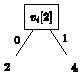
\includegraphics[scale=2.5]{chapters/mining/mining-ethereum-figures/dectree.pdf}
\end{minipage}
\caption{The classification problem is based on the gas used by $\tx_3$ (left) and the resulting decision tree (right).} 
\label{fig:mining-ethereum-dectree}
\end{figure}


\paragraph{Step (3): Extracting Gas Usage Rules} Now that we have estimated the neighborhood of every transaction, our next goal is to extract a set of rules that define the gas usage of each transaction $\tx$ based on the subset of neighbors that precede $\tx$ in the block and their order of appearance.


\paragraph{Syntax} Our rules are defined by the grammar below:
\begin{equation} \label{eq:ethereum-mining-grammar}
\begin{matrix*}[l]
\langle \text{predicate} \rangle & :=  &   \has \tx ~|~  \tx \before \tx ~|~ \neg \langle \text{predicate} \rangle \\
\langle \text{predicate-list} \rangle & :=  & \langle \text{predicate} \rangle ~|~ \langle \text{predicate} \rangle, \langle \text{predicate-list} \rangle    \\
\langle \text{clause} \rangle  & := &  \langle \text{predicate} \rangle ~|~  \atleast(k, \langle \text{predicate-list} \rangle) ~|~\\
& &  \langle \text{clause} \rangle \land \langle \text{clause} \rangle \\
\langle \text{rule} \rangle & := & \langle \text{clause} \rangle  \Rightarrow \expgas(\tx) = g\\
& &g, k \in \mathbb N, \tx \in \pool
\end{matrix*}
\end{equation}



\paragraph{Semantics} Given a sequence of distinct transactions $\pi = \langle \pi[1], \ldots, \pi[m]\rangle, $ we have:
\begin{equation} \label{eq:ethereum-mining-semantics}
\begin{matrix*}[l]
	\pi \models \has\tx_i & \Leftrightarrow & \exists i' ~~ (\pi[i'] = \tx_i) \\
	 \pi \models \tx_i \before \tx_j & \Leftrightarrow & \pi \not\models \has\tx_j \lor \exists i', j' ~~ (i'<j' \land  \\
	 &&\pi[i'] = \tx_i \land \pi[j'] = \tx_j)\\

	 \pi \models \neg p & \Leftrightarrow & \pi \not\models p\\
	 \pi \models c_1 \land c_2 & \Leftrightarrow & \pi \models c_1 \land \pi \models c_2\\
	 \pi \models \atleast(k, p_1, \ldots, p_m) & \Leftrightarrow & \exists i_1, \ldots, i_k ~~ (1 \leq i_1 < \ldots < i_k \leq m \land \\
	 &&\forall j ~~ \pi \models p_{i_j})
\end{matrix*}
\end{equation}

Intuitively, $\pi$ satisfies the predicate $\has \tx_i$ if it includes $\tx_i.$ It satisfies the predicate $\tx_i \before \tx_j$ if it either excludes $\tx_j$ altogether or has $\tx_i$ preceding $\tx_j.$ A clause is simply a conjunction of predicates. We also allow clauses of the form $\atleast(k, p_1, \ldots, p_m)$ which require $\pi$ to satisfy at least $k$ of the predicates $p_1, \ldots, p_m.$ Although the latter could be left as syntactic sugar, including it as a separate clause is helpful in practice. This is because of a common scenario in smart contracts, especially those modeling NFT or token giveaways, in which the first $k$ transactions to call a function can receive the token. In such cases, all transactions calling this function are dependent in terms of gas, but the gas usage of each of them is only dependent on how many other transactions precede it.  Finally, a rule of the form $C \Rightarrow \expgas(\tx_i) \geq g$ signifies a prediction: if $C$ is satisfied, we expect the gas usage of the transaction $\tx_i$ to be at least $g.$



\paragraph{Step (3.i): Generating a Decision Tree}  In this step, we generate a set of rules for each transaction $\tx_i \in \pool.$ We process each such transaction separately. When generating the rules for $\tx_i,$ we narrow our focus down to its neighborhood $\nbhd(\tx_i)$ since we believe these are the only transactions that can affect the gas usage of $\tx_i.$ Let $\pi_j$ be one of the sample permutations. We define $\pi_j^*$ as the subsequence of $\pi_j$ induced by $\nbhd(\tx_i) \cup \{\tx_i\},$ i.e.~the subsequence obtained by removing every element that is not in the neighborhood or not $\tx_i$ itself. If $\pi \not\models \has \tx_i,$ we ignore this sample as it does not include $\tx_i$ and cannot give us any information about its gas usage. We use $\Pi^*$ to denote the set of neighborhood-induced samples.
 
 As in Step 2, our goal is to form a decision tree that predicts the gas usage of $\tx_i$ based on features that encode the set of neighbors that precede it in the block and their order. Thus, for every neighboring $\tx_j \in \nbhd(\tx_i)$ we define a corresponding feature
 $$
 w[j] = \left\{ 
 	\begin{matrix}
 		j' - i' &  \text{if }\pi^* \models \tx_j \before \tx_i \land \pi^*[i']=\tx_i  \land \pi^*[j'] = \tx_j \\
 		0 & \text{otherwise}
 	\end{matrix}
 	\right..
 $$   
 Informally, if $\pi^*$ puts $\tx_j$ before $\tx_i,$ then $-w[j]$ is the distance between the two transactions in $\pi^*.$ Otherwise, $w[j]=0.$ In other words, we care about the distance only if $\tx_j$ precedes $\tx_i.$ This is because if $\tx_j$ does not appear before $\tx_i,$ it cannot affect $\tx_i$'s gas usage.  In addition to the $w[j]$'s, we also add an extra feature $r$ which models the number of neighbors that precede $\tx_i,$ or equivalently, the index in $\pi^*$ at which $\tx_i$ appears. We generate a decision tree using the same method as in Step 2, where the samples are the subsequences $\pi^*,$ the features are $r$ and the $w[j]$'s, and the labels are different possible gas usage values of $\tx_i.$ Note that our features are no longer binary. 

% Questions: Why do we need r? Why did we come up with this vectors?

\paragraph{Example} For step 2 of the algorithm in our previous example, suppose we know that $\nbhd(\tx_1) = \{\tx_4, \tx_5\}$. Then for $\pi_1 = \langle \tx_4,\tx_5, \tx_1, \tx_2, \tx_3, \tx_6\rangle$ the induced sample is $\pi_1^* = \langle \tx_4, \tx_5, \underline{\tx_1} \rangle.$ The encoding $w[\tx_4] = 0 - 2$ as the position of $\tx_4$ is $0$ and the position of $\tx_1$ is $2.$ Similarly, $w[\tx_5] = 1 - 2 = -1$ and $w[\tx_1] = 2 - 2 = 0.$ The feature $w[r] = 2$ as the number of neighbors that precede $\tx_1$ is $2.$ The encoding of the rest of the samples is shown in Figure~\ref{fig:mining-ethereum-dectree-2}.


\newcommand{\fmmmm}{\mspace{1mu}} %fake minus
\newcommand{\fmmm}{\mspace{2mu}} %fake minus


\newcommand{\fm}{\mspace{12mu}} %fake minus
\newcommand{\fmm}{\mspace{11mu}} %fake minus

\newcommand{\fmz}{\mspace{9mu}} %fake minus
\newcommand{\fma}{\mspace{10mu}} %fake minus
\newcommand{\fmb}{\mspace{11mu}} %fake minus
\newcommand{\fmc}{\mspace{12mu}} %fake minus
\newcommand{\fmd}{\mspace{13mu}} %fake minus
\newcommand{\fme}{\mspace{14mu}} %fake minus

\begin{figure}
\centering
{
\small
\begin{tabular}{|c|c|c|c|}
\hline
\shortstack{Sample\\($\pi_i$)} & \shortstack{nbhd($\tx_1$)-induced \\ Sample ($\pi^*_i$)} & \shortstack{Encoding ($w$)\\$|\pi_1, \pi_4, \pi_5, r\mspace{1mu}|$} & \shortstack{Label\\$(\tx_1$'s gas)}\\ \hline\hline
$\pi_1$    & $\langle\tx_4, \tx_5, \underline{\tx_1} \rangle$ &  $[0,   -2,    -1,2]$       & $ 6$\\
$\pi_2$    & $\langle\tx_4, \underline{\tx_1}, \tx_5 \rangle$ &  $[0,   -1, \fmb 0,1]$      & $ 8$\\
$\pi_3$    & $\langle\underline{\tx_1}, \tx_5, \tx_4 \rangle$ &  $[0,\fmb 0,\fmb 0,0]$      & $10$\\
$\pi_4$    & $\langle\tx_4, \underline{\tx_1}, \tx_5 \rangle$ &  $[0,   -1, \fmb 0,1]$      & $ 8$\\
$\pi_5$    & $\langle\tx_4, \tx_5, \underline{\tx_1} \rangle$ &  $[0,   -2,    -1,2]$       & $ 6$\\
$\pi_6$    & $\langle\tx_4, \underline{\tx_1}, \tx_5 \rangle$ &  $[0,  \fmmm -1, \fma 0,1]$ & $ 8$\\
$\pi_7$    & $\langle\tx_5, \underline{\tx_1}, \tx_4 \rangle$ &  $[0,\fm 0,    -1,1]$       & $ 2$\\
$\pi_8$    & $\langle\underline{\tx_1}, \tx_4, \tx_5 \rangle$ &  $[0,\fmb 0,\fmc 0,0]$      & $10$\\
$\pi_9$    & $\langle\tx_5, \underline{\tx_1}, \tx_4 \rangle$ &  $[0,\fm 0,   -1,  1]$        & $ 2$\\
$\pi_{10}$ & $\langle\underline{\tx_1}, \tx_5, \tx_4 \rangle$ &  $[0,\fmb 0,\fmc 0,0]$      & $10$\\ 
\hline
\end{tabular}
}
\caption{The classification problem  based on the gas used by $\tx_1$}
\label{fig:mining-ethereum-dectree-2}
\end{figure}




\paragraph{Step (3.ii): Extracting Rules from the Decision Tree} In the decision tree generated for $\tx_i$ in Step (3.i), every leaf is labeled by one possible gas usage value of $\tx_i.$ Let $\ell$ be a leaf labeled by $g_\ell$. Consider a feature $w[j].$ We know that $-n \leq w[j] \leq 0.$ In the path from the root of the decision tree to the leaf $\ell,$ some decisions bound $w[j]$ from above or below. Let $m_j$ be the largest lower-bound and $M_j$ the smallest upper-bound imposed on $w[j]$ in the root-to-leaf path ending at $\ell.$ Thus, in all samples modeled by this leaf, we have $w[j] \in [m_j, M_j].$ Similarly, we can define the tightest possible segment $[m_r, M_r]$ for values of $r$ in these samples. For each leaf $\ell,$ we generate a gas usage rule containing a clause $\varphi_\ell$ as follows:
\begin{itemize}
	\item We add the conjunct $\has \tx_i$ to $\varphi_\ell.$
	\item If for two transactions $\tx_j, \tx_{j'} \in \nbhd(\tx_i),$ we have $M_j \leq m_{j'},$ then $\tx_j$ is always preceding $\tx_{j'}$ in the samples corresponding to $\ell.$ Thus, we add the conjunct $\tx_j \before \tx_{j'}$ to $\varphi_\ell.$ 
	\item If for a transaction $\tx_j \in \nbhd(\tx_i),$ we have $m_j \geq 0,$ then $\tx_j$ is never appearing before $\tx_i$ in the samples corresponding to $\ell.$ Thus, we add the conjunct $\tx_i \before \tx_j$ to $\varphi_\ell.$
	\item If $m_r > 0,$ then in every sample corresponding to $\ell,$ at least $m_r$ neighboring transactions preceded $\tx_i.$ Let the neighborhood of $\tx_i$ be $\nbhd(\tx_i) = \{\tx_{j, 1}, \ldots, \tx_{j, q}\}.$ To capture this, we add the conjunct $\atleast(m_r, \tx_{j, 1} \before \tx_i, \ldots, \tx_{j, q} \before \tx_i)$ to $\varphi_\ell.$ 
	\item Similarly, if $\nbhd(\tx_i) = \{\tx_{j, 1}, \ldots, \tx_{j, q}\}$ and $M_r < q,$ then at most $M_r$ neighbors precede $\tx_i$ in each of the samples corresponding to $\ell.$ Therefore, $\tx_i$ precedes at least $q-M_r$ neighbors in each such sample. Hence, we add the conjunct $\atleast(q-M_r, \tx_i \before \tx_{j, 1}, \ldots, \tx_i \before \tx_{j, q})$ to the clause $\varphi_\ell.$
\end{itemize}
By definition-chasing, it is easy to prove that for every sample $\pi^*$ corresponding to the leaf $\ell$ of the decision tree, we have $\pi^* \models \varphi_\ell.$ Hence, one might assume that the expected gas usage of $\tx_i$ in a sample satisfying $\varphi_\ell$ is the same as $\ell$'s label $g_\ell.$ However, $\varphi_\ell$ might be satisfied by other samples, i.e.~samples corresponding to other leaves, too. This is rare in practice, but to handle it, our algorithm takes the average gas usage of $\tx_i$ over \emph{all} samples $\pi^*$ that model $\varphi_\ell.$ Formally, let $J = \{ j ~|~ 1 \leq j \leq k  \land \pi^*_j \models \varphi_\ell \}.$ Our algorithm computes
$$
\overline{g}_\ell = \frac{\sum_{j \in J} \gas(\pi_j, \tx_i) }{|J|}.
$$
In almost all real-world cases, we have $\overline{g}_\ell = g_\ell.$ Finally, our algorithm generates the following gas usage rule:
\begin{equation} \label{eq:mining-ethereum-gur}
\varphi_\ell \Rightarrow \expgas(\tx_i) = \overline{g}_\ell.
\end{equation}
We remark that for each transaction $\tx_i$ and every leaf $\ell$ of the decision tree corresponding to $\tx_i,$ our algorithm generates one instance of the gas usage rule in Equation~\eqref{eq:mining-ethereum-gur}.

\paragraph{Example} Let Figure \ref{fig:mining-ethereum-dectree-final} be the decision tree generated for $\tx_1$ in our previous example. The tree has $6$ leaves $l_1$ -- $l_6$ labelled $10, 2, 10, 8, 6, 6$ respectively. Consider the leaf $l_5$, taking the negations into the account, the predicates along the path evaluate to: $w[\pi_4] < 0.0$, $w[\pi_5] \geq -1.5$, $w[\pi_4] < -1.5$, which after rounding to integers, gives us the intervals $w[\pi_4] \in (-\infty, -2] = (m_4, M_4]$, $w[\pi_5] \in [-1, \infty) = [m_5, M_5)$. Notice that $M_4 \leq 0$ which generates the clause $\tx_4 \before tx_1$, and $M_4 \leq m_5$ which generates the clause $\tx_4 \before \tx_5$. Therefore, the rule's body is $\has \tx_1 \land (\tx_4 \before \tx_1) \land (\tx_4 \before \tx_5)$. Observe that  $\{\pi_1, \pi_2, \pi_4, \pi_5, \pi_6\} \models \has \tx_1 \land (\tx_4 \before \tx_1) \land (\tx_4 \before \tx_5)$, with average gas usage of $\tx_1$ equal to $(6 + 8 + 8 + 6 + 8)/5 = 7.2$. The remaining rules are given in Figure \ref{fig:mining-ethereum-rules}. 

Notice that no permutation can satisfy the rule $l_4$ and we assign the undefined $\bot$ average usage to it. We exclude such rules from consideration in the rest of the algorithm.


\begin{figure}
\centering
\begin{forest}
[
$w {[\pi_4]}$ $ \geq 0.0$
	[
	$w{[\pi_5]}$ $ \geq 0.0$
		[$l_1$: $10$]
		[$l_2$: $2$]
	]
	[
	$w{[\pi_5]}$ $ \geq -1.5$
		[
		$w{[\pi_4]}$ $ \geq -1.5$
			[$w{[\pi_5]}$ $ \geq 0.0$
			[$l_3$: $8$]
			[$l_4$: $6$]
			]
			[$l_5$: $6$]
		]
		[$l_6$: $6$]
	]
]
\end{forest}
\caption{The resulting decision tree for $\tx_1$.}
\label{fig:mining-ethereum-dectree-final}
\end{figure}

\begin{figure}
    \newcommand{\shiftleft}{\mspace{-50mu}} 

    \begin{equation*} 
        \begin{matrix}
            & m_4,M_4 & m_5,M_5 && \textup{rule} & & \shiftleft \expgas(\tx_1)\\
l_1: & [0, \infty)& [0, \infty) && \has \tx_1 \land (\tx_1 \before \{\tx_4, \tx_5\})& \Rightarrow &  10 \\
l_2: & [0, \infty)& (-\infty, -1] && \has \tx_1 \land (\tx_1 \before \tx_4) \land (\tx_5 \before \tx_1) & \Rightarrow &  2 \\
l_3: & [-1, -1]& [0, \infty) && \has \tx_1 \land (\tx_4 \before \tx_1) \land (\tx_1 \before \tx_5) & \Rightarrow &  8 \\
l_4: & [-1, -1]& [-1, -1] && \has \tx_1\land (\{\tx_4,\tx_5\} \before \tx_1)\land   & \Rightarrow &  \bot \\
&&&&(\tx_4 \before \tx_5) \land (\tx_5 \before \tx_4) && \\
l_5: & (-\infty, -2]& [-1, \infty) && \has \tx_1 \land (\tx_4 \before \tx_1) \land (\tx_4 \before \tx_5) & \Rightarrow &  7.2 \\
l_6: & (-\infty, -1]& (-\infty, -2] && \has \tx_1 \land (\{\tx_4, \tx_5\} \before \tx_1)  & \Rightarrow &  6 \\
\end{matrix}
\end{equation*}
\caption{The gas usage rules generated for $\tx_1$.}
\label{fig:mining-ethereum-rules}
\end{figure}


\begin{theorem}
	\label{thm:mining-ethereum-sufficient-samples}
	
	Assume there are no nonce dependencies and the neighborhood of every transaction is known. Consider the following stochastic process: We start with an empty sample set. In each step, we uniformly sample a new permutation of the transactions in $\pool$ and add it to $\Pi$. The process stops at the moment $T$ when the sample set $\Pi$ becomes sufficient. Then,  for any $\varepsilon \in (0, 1)$, the following holds:
	\[
        \PP{T < \Delta! \cdot \log \frac{|\pool| \cdot (\Delta + 1)!}{\varepsilon}} \geq 1 - \varepsilon.
	\]
\end{theorem}
\begin{proof}[Proof of \Cref{thm:mining-ethereum-sufficient-samples}]
For a transaction $\tx$, the probability that an induced permutation $\pi^*$ does not appear after one step is 
$
1 - \frac{1}{(|\nbhd(\tx)| + 1)!} \leq 1 - \frac{1}{(\Delta + 1)!}.
$
By the independence of trials, the probability that the induced permutation remains unseen after $r$ steps is 
$
\left(1 - \frac{1}{(\Delta + 1)!}\right)^r \leq \exp\left(-\frac{r}{(\Delta + 1)!}\right).
$
As for each $\tx$ there are at most $(\Delta + 1)!$ induced blocks, by the union bound, the probability that there exists a transaction $\tx$ such that the induced permutation $\pi^*$ does not appear after $r$ steps is at most 
$
	\PP{T \geq r} \leq |\pool| \cdot (\Delta + 1)! \cdot \exp\left(-\frac{r}{(\Delta + 1)!}\right).
$
After plugging in
$
r = (\Delta + 1)! \cdot \log \left(\frac{|\pool| \cdot (\Delta + 1)!}{\varepsilon}\right),
$
and rearranging the terms, we obtain the desired result.

\end{proof}	

\section{Runtime and Revenue Results on Ethereum}\label{sec:mining-ethereum-experiments}

\paragraph{Implementation}
We implemented our approach in Python 3 and Rust. Our tool is open-access and available online. We used Anvil~\cite{foundry2023anvil} and Erigon~\cite{erigontech2023erigon} to execute Ethereum transactions in our samples and to obtain their gas usage. Moreover, we used Linfa~\cite{linfa2025linfa} to generate decision trees and relied on SCIP~\cite{bolusani2024scip} to solve Integer Linear Programming (ILP) instances.


\paragraph{Machine} All experimental results were obtained on an Intel Xeon Gold 5115 Machine (2.40GHz, 16 cores) with 64 GB of RAM, running Ubuntu 22.04.

\paragraph{Benchmarks}
As our benchmark suite, we collected a dataset of real-world mempools, i.e.~ unmined transactions, that were available on the Ethereum network before each block. Our data spans 50,000 blocks, numbered 21800000 to 21849999, corresponding to approximately one week of activity on Ethereum in the period from February 8, 2025, 06:27:11 (UTC) to February 15, 2025, 06:18:35 (UTC). This data was gathered from Blocknative~\cite{blocknative2025mempool}. 

\paragraph{Samples and Runtime} For each of the 50,000 blocks, we generated 300 sample permutations and limited our solver's execution time to 12 seconds, i.e.~Ethereum's block time. We note that the results were obtained on a relatively modest machine. The testing and decision-tree generation steps of our algorithm are parallelized, thus increasing the computational power would allow one to cover more samples for each block. We expect real-world miners to have much higher computational power than us.

\paragraph{Baselines} For each block, we compare the total tip revenue obtained by our approach with the real-world block that was mined and added to the Ethereum blockchain. In the experiments, we observed that some Ethereum miners routinely miss lucrative transactions when forming their blocks. This might be due to a suboptimal block formation strategy or network connectivity issues that prevented the miner from seeing the transactions, e.g.~due to the censorship of the Ethereum network in some countries. Thus, it is conceivable that the miner might not have the same mempool as us. We believe this does not affect the fairness of the comparison since the onus is on the miners to ensure they have reliable connectivity to the network. However, to demonstrate that our improvements are not merely due to better connectivity, as a second baseline, we used Ethereum's reference implementation and applied it to the exact same mempools as our algorithm. The reference implementation sorts transactions greedily based on their effective gas tip value, prioritizing transactions with higher tips for miners and ordering same-sender transactions by nonce~\cite{foundry2023anvil, foundation2025go}.




\begin{table}[!htbp]
\centering
\caption{Improvements obtained by our approach compared to real-world miners and the Ethereum reference implementation.}
\label{table:mining-ethereum-comparisonBaseline}
\renewcommand{\arraystretch}{1.2}
\begin{tabular}{|>{\raggedright\arraybackslash}p{0.32\textwidth}|>{\raggedright\arraybackslash}p{0.32\textwidth}|>{\raggedright\arraybackslash}p{0.32\textwidth}|}
\hline
\textbf{Metric} & Improvement compared to Real-World Miners & Improvement compared to Reference Implementation \\
\hline\hline
Number of improved blocks & 45{,}609 (91.22\%) & 38{,}505 (77.01\%) \\ \hline
Total increase in tip revenue over 50{,}000 blocks & 1{,}204{,}475 USD & 863{,}385 USD \\ \hline
Annualized increase in tip revenue & 63{,}357{,}892 USD & 45{,}416{,}764 USD \\ \hline
Average earning increase per block & 24.1 USD & 17.3 USD \\ \hline
Average improvement percentage per block & 73.45\% & 18.56\% \\ 
\hline
\end{tabular}
\renewcommand{\arraystretch}{1}
\end{table}

% Question why going from 18 percent to 73 percent does not make a huge different in USD?

\paragraph{Revenue Gains}
 The revenue gains obtained by our algorithm are summarized in Table~\ref{table:mining-ethereum-comparisonBaseline} and Figure~\ref{fig:mining-ethereum-revenueComparisionWReal}. Our approach outperformed real-world miners in 45,609 of the 50,000 blocks (91\% of the cases), increasing the total revenue over all blocks by \textbf{1,204,475 USD}\footnote{We used the ETH/USD conversion rates provided by~\cite{coinmarketcap2025cryptocurrency}.}. On average, this represents an increase of nearly 24.1 USD per block, which translates to an annualized improvement of around \textbf{63 million USD} . Our approach obtained significant gains compared to the Ethereum reference implementation, as well. It outperformed the reference implementation in 38,505 blocks (77\% of the cases), yielding an additional revenue of \textbf{863,385 USD} over our 50,000 benchmark blocks. This translates to approximately \textbf{45 million USD} annually. On average, our algorithm earned almost 17.3 USD more per block. The data in Table~\ref{table:mining-ethereum-comparisonBaseline} should be taken with the usual grains of salt: (i)~Ether's value and its exchange rate to USD are highly volatile and unpredictable, and (ii)~the reported numbers are the sums of improvements over individual blocks. Figures~\ref{fig:mining-ethereum-revenueIncreaseReal} and~\ref{fig:mining-ethereum-revenueIncreaseGreedy} and provide histograms of the gained revenues in USD.  Figures~\ref{fig:mining-ethereum-percentageImprovementOverReal} and~\ref{fig:mining-ethereum-percentageImprovementOverGreedy} show similar histograms based on the percentage of improvement obtained in each block.



 \begin{figure}[ht]
	\centering
	\includegraphics[width=0.6\columnwidth]{chapters/mining/mining-ethereum-figures/revenueComparisionWReal.pdf}
	\caption{
		Comparison of the tip revenues obtained by our algorithm (x-axis) and the real-world blocks added to the Ethereum blockchain (y-axis). Each point corresponds to one block. Green points (91.22\%) are the blocks on which our algorithm obtained a higher revenue than real-world miners. For clarity, we excluded 265 data points.} 
	\label{fig:mining-ethereum-revenueComparisionWReal}
\end{figure}


\begin{figure}[ht]
	\centering
	\includegraphics[width=0.8\columnwidth]{chapters/mining/mining-ethereum-figures/revenueImprovementReal.pdf}
	\caption{Histogram of the transaction fee improvements obtained over each block compared to real-world miners (in USD). The y-axis is in logarithmic scale. For clarity, 411 data points outside the range are omitted.}
	\label{fig:mining-ethereum-revenueIncreaseReal}
\end{figure}



\begin{figure}[ht]
    \centering
    \includegraphics[width=0.8\columnwidth]{chapters/mining/mining-ethereum-figures/revenueImprovementGreedy.pdf}
    \caption{Histogram of the transaction fee improvements obtained over each block compared to the Ethereum reference implementation (in USD). The y-axis is in logarithmic scale. For readability, 868 blocks with improvements over 150 USD are omitted from the plot.}
    \label{fig:mining-ethereum-revenueIncreaseGreedy}
\end{figure}


\begin{figure}[ht]
	\centering
	\includegraphics[width=0.8\columnwidth]{chapters/mining/mining-ethereum-figures/percentageImprovementOverReal.pdf}
	\caption{Histogram of the transaction fee improvements obtained over each block compared to real-world miners (in percentages). 608 points outside the range omitted for clarity.}
	\label{fig:mining-ethereum-percentageImprovementOverReal}
\end{figure}



\begin{figure}[ht]
    \centering
    \includegraphics[width=0.8\columnwidth]{chapters/mining/mining-ethereum-figures/percentageImprovementOverGreedy.pdf}
    \caption{Histogram of the transaction fee improvements obtained over each block compared to the Ethereum reference implementation (in percentages). The y-axis is in logarithmic scale. 2021 points outside the range omitted for clarity.}
    \label{fig:mining-ethereum-percentageImprovementOverGreedy}
\end{figure}



\paragraph{Sample Size Sensitivity} To investigate the effect of sample size on our approach, we reran our experiments with sample sizes of $50$, $100$, $200$, and $300$. The improvement in revenue slows as sample size increases. We observed that the marginal gain from $200$ to $300$ samples is less pronounced. See Table~\ref{table:mining-ethereum-parametersensitivity} for details. Moreover, the average neighborhood size is $1.21$, which, according to Theorem~\ref{thm:mining-ethereum-sufficient-samples}, indicates that relatively small sample sizes suffice.

\begin{table}
\centering

\caption{Pairwise differences in annualized revenue across sample sizes of 50, 100, 200, and 300 in thousands of USD.}

\label{table:mining-ethereum-parametersensitivity}
\begin{tabular}{|c|c|c|c|c|}
\hline
\makecell{\textbf{Sample Size}} & \makecell{\textbf{50}} & \makecell{\textbf{100}} & \makecell{\textbf{200}} & \makecell{\textbf{300}} \\
\hline\hline
50 & 0 & -1457.53 & -2910.24 & -3253.29 \\
\hline
100 & 1457.53 & 0 & -1452.71 & -1795.76 \\
\hline
200 & 2910.24 & 1452.71 & 0 & -343.047 \\
\hline
300 & 3253.29 & 1795.76 & 343.047 & 0 \\
\hline
\end{tabular}

\end{table}



\paragraph{Runtime Performance} In practice, executing one block sample took 2.42 seconds on average. The end-to-end processing took an average of 5.7 seconds (without parallelization). Moreover, the pure ILP solving time (Step 5) was only 0.4 seconds.
Refer to Figures~\ref{fig:mining-ethereum-HistogramIlpOnEndToEndOverlay} for details.
We emphasize that steps 2-4 can be parallelized, allowing for runtime reduction with additional computational power. The ILP performance depends primarily on instance sparsity rather than mempool size. We observed that increasing the number of transactions in the mempool leads to ILP instances that are easier and faster to solve. See Figure~\ref{fig:mining-ethereum-ScatterIlpTimeTxCountSampleSize300} for details.



\begin{figure}[ht]
    \centering
    \includegraphics[width=0.8\columnwidth]{chapters/mining/mining-ethereum-figures/HistogramIlpOnEndToEndOverlay.pdf}
	\caption{Histogram of the end-to-end (green) and ILP solver (blue) processing times per block. The y-axis is in logarithmic scale.}
	\label{fig:mining-ethereum-HistogramIlpOnEndToEndOverlay}
\end{figure}


\begin{figure}[ht]
	\centering
	\includegraphics[width=0.8\columnwidth]{chapters/mining/mining-ethereum-figures/ScatterIlpTimeTxCountSampleSize300.pdf}
	\caption{Scatter of ILP solver time (seconds) versus number of transactions per mempool, with sample size fixed at 300.}
	\label{fig:mining-ethereum-ScatterIlpTimeTxCountSampleSize300}
\end{figure}


% \begin{figure}[h]
% 	\centering
% 	\begin{subfigure}[b]{0.48\textwidth}
% 		\centering
% 		\includegraphics[width=\textwidth]{chapters/mining/mining-ethereum-figures/ScatterIlpTimeTxCountSampleSize50.pdf}
% 		\subcaption{Sample size 50}
% 		\label{fig:ScatterIlpTimeTxCountSampleSize50}
% 	\end{subfigure}
% 	\hfill
% 	\begin{subfigure}[b]{0.48\textwidth}
% 		\centering
% 		\includegraphics[width=\textwidth]{chapters/mining/mining-ethereum-figures/ScatterIlpTimeTxCountSampleSize100.pdf}
% 		\subcaption{Sample size 100}
% 		\label{fig:ScatterIlpTimeTxCountSampleSize100}
% 	\end{subfigure}
	
% 	\begin{subfigure}[b]{0.48\textwidth}
% 		\centering
% 		\includegraphics[width=\textwidth]{chapters/mining/mining-ethereum-figures/ScatterIlpTimeTxCountSampleSize200.pdf}
% 		\subcaption{Sample size 200}
% 		\label{fig:ScatterIlpTimeTxCountSampleSize200}
% 	\end{subfigure}
% 	\hfill
% 	\begin{subfigure}[b]{0.48\textwidth}
% 		\centering
% 		\includegraphics[width=\textwidth]{chapters/mining/mining-ethereum-figures/ScatterIlpTimeTxCountSampleSize300.pdf}
% 		\subcaption{Sample size 300}
% 		\label{fig:ScatterIlpTimeTxCountSampleSize300A}
% 	\end{subfigure}
	
% 	\caption{\added{Scatter of ILP solver time (seconds) versus number of transactions per mempool for different sample sizes.}}
% 	\label{fig:ScatterIlpTimeTxCount}
% \end{figure}

% \clearpage
% \begin{figure}[h]
% 	\centering
% 	\begin{subfigure}[b]{0.48\textwidth}
% 		\centering
% 		\includegraphics[width=\textwidth]{chapters/mining/mining-ethereum-figures/ScatterIlpTimeByAvgNeighborhoodSampleSize50.pdf}
% 		\subcaption{Sample size 50}
% 		\label{fig:ScatterIlpTimeByAvgNeighborhoodSampleSize50A}
% 	\end{subfigure}
% 	\hfill
% 	\begin{subfigure}[b]{0.48\textwidth}
% 		\centering
% 		\includegraphics[width=\textwidth]{chapters/mining/mining-ethereum-figures/ScatterIlpTimeByAvgNeighborhoodSampleSize100.pdf}
% 		\subcaption{Sample size 100}
% 		\label{fig:ScatterIlpTimeByAvgNeighborhoodSampleSize100A}
% 	\end{subfigure}
	
% 	\begin{subfigure}[b]{0.48\textwidth}
% 		\centering
% 		\includegraphics[width=\textwidth]{chapters/mining/mining-ethereum-figures/ScatterIlpTimeByAvgNeighborhoodSampleSize200.pdf}
% 		\subcaption{Sample size 200}
% 		\label{fig:ScatterIlpTimeByAvgNeighborhoodSampleSize200A}
% 	\end{subfigure}
% 	\hfill
% 	\begin{subfigure}[b]{0.48\textwidth}
% 		\centering
% 		\includegraphics[width=\textwidth]{chapters/mining/mining-ethereum-figures/ScatterIlpTimeByAvgNeighborhoodSampleSize300.pdf}
% 		\subcaption{Sample size 300}
% 		\label{fig:ScatterIlpTimeByAvgNeighborhoodSampleSize300A}
% 	\end{subfigure}
	
% 	\caption{\added{Scatter of ILP solver time (seconds) versus average neighborhood size per block for different sample sizes.}}
% 	\label{fig:ScatterIlpTimeByAvgNeighborhood}
% \end{figure}

% \begin{figure}[h]
% 	\centering
% 	\begin{subfigure}[b]{0.48\textwidth}
% 		\centering
% 		\includegraphics[width=\textwidth]{chapters/mining/mining-ethereum-figures/HistogramNeighborhoodSizeSampleSize50.pdf}
% 		\subcaption{Sample size 50}
% 		\label{fig:HistogramNeighborhoodSizeSampleSize50A}
% 	\end{subfigure}
% 	\hfill
% 	\begin{subfigure}[b]{0.48\textwidth}
% 		\centering
% 		\includegraphics[width=\textwidth]{chapters/mining/mining-ethereum-figures/HistogramNeighborhoodSizeSampleSize100.pdf}
% 		\subcaption{Sample size 100}
% 		\label{fig:HistogramNeighborhoodSizeSampleSize100A}
% 	\end{subfigure}
	
% 	\begin{subfigure}[b]{0.48\textwidth}
% 		\centering
% 		\includegraphics[width=\textwidth]{chapters/mining/mining-ethereum-figures/HistogramNeighborhoodSizeSampleSize200.pdf}
% 		\subcaption{Sample size 200}
% 		\label{fig:HistogramNeighborhoodSizeSampleSize200A}
% 	\end{subfigure}
% 	\hfill
% 	\begin{subfigure}[b]{0.48\textwidth}
% 		\centering
% 		\includegraphics[width=\textwidth]{chapters/mining/mining-ethereum-figures/HistogramNeighborhoodSizeSampleSize300.pdf}
% 		\subcaption{Sample size 300}
% 		\label{fig:HistogramNeighborhoodSizeSampleSize300A}
% 	\end{subfigure}
	
% 	\caption{\added{Histogram of neighborhood size per block for different sample sizes.}}
% 	\label{fig:HistogramNeighborhoodSize}
% \end{figure}